\documentclass[10pt]{beamer}
\usepackage{amsmath}
\usepackage{mathtools}
\usepackage{multimedia}
\usepackage{hyperref}


\usefonttheme{professionalfonts} % using non standard fonts for beamer
\usefonttheme{serif} % default family is serif
%\documentclass[12pt]{beamerthemeSam.sty}
\usepackage{epsf}
%\usepackage{pstricks}
%\usepackage[orientation=portrait,size=A4]{beamerposter}
\geometry{paperwidth=160mm,paperheight=120mm}
%DT favorite definitions
\def\LL{\left\langle}	% left angle bracket
\def\RR{\right\rangle}	% right angle bracket
\def\LP{\left(}		% left parenthesis
\def\RP{\right)}	% right parenthesis
\def\LB{\left\{}	% left curly bracket
\def\RB{\right\}}	% right curly bracket
\def\PAR#1#2{ {{\partial #1}\over{\partial #2}} }
\def\PARTWO#1#2{ {{\partial^2 #1}\over{\partial #2}^2} }
\def\PARTWOMIX#1#2#3{ {{\partial^2 #1}\over{\partial #2 \partial #3}} }

\def\rightpartial{{\overrightarrow\partial}}
\def\leftpartial{{\overleftarrow\partial}}
\def\diffpartial{\buildrel\leftrightarrow\over\partial}

\def\BC{\begin{center}}
\def\BS{\bigskip}
\def\EC{\end{center}}
\def\BN{\begin{enumerate}}
\def\EN{\end{enumerate}}
\def\BI{\begin{itemize}}
\def\EI{\end{itemize}}
\def\BE{\begin{displaymath}}
\def\EE{\end{displaymath}}
\def\BEA{\begin{eqnarray*}}
\def\EEA{\end{eqnarray*}}
\def\BNEA{\begin{eqnarray}}
\def\ENEA{\end{eqnarray}}
\def\EL{\nonumber\\}

\newcommand{\etal}{{\it et al.}}
\newcommand{\gbeta}{6/g^2}
\newcommand{\la}[1]{\label{#1}}
\newcommand{\ie}{{\em i.e.\ }}
\newcommand{\eg}{{\em e.\,g.\ }}
\newcommand{\cf}{cf.\ }
\newcommand{\etc}{etc.\ }
\newcommand{\atantwo}{{\rm atan2}}
\newcommand{\Tr}{{\rm Tr}}
\newcommand{\dt}{\Delta t}
\newcommand{\op}{{\cal O}}
\newcommand{\msbar}{{\overline{\rm MS}}}
\def\chpt{\raise0.4ex\hbox{$\chi$}PT}
\def\schpt{S\raise0.4ex\hbox{$\chi$}PT}
\def\MeV{{\rm Me\!V}}
\def\GeV{{\rm Ge\!V}}

%AB: my color definitions
%\definecolor{mygarnet}{rgb}{0.445,0.184,0.215}
%\definecolor{mygold}{rgb}{0.848,0.848,0.098}
%\definecolor{myg2g}{rgb}{0.647,0.316,0.157}
\definecolor{A}{rgb}{1.0,0.3,0.3}
\definecolor{B}{rgb}{0.0,1.0,0.0}
\definecolor{C}{rgb}{1.0,1.0,0.0}
\definecolor{D}{rgb}{0.5,0.5,1.0}
\definecolor{E}{rgb}{0.7,0.7,0.7}
\definecolor{abtitlecolor}{rgb}{1.0,1.0,1.0}
\definecolor{absecondarycolor}{rgb}{0.0,0.416,0.804}
\definecolor{abprimarycolor}{rgb}{1.0,0.686,0.0}
\definecolor{Red}           {rgb}{1,0.4,0.4}
\definecolor{Yellow}           {rgb}{1,1,0.0}
\definecolor{Grey}          {cmyk}{.7,.7,.7,0}
\definecolor{Blue}          {cmyk}{1,1,0,0}
\definecolor{Green}         {cmyk}{1,0,1,0}
\definecolor{Brown}         {cmyk}{0,0.81,1,0.60}
\definecolor{Silver}        {rgb}{0.95,0.9,1.0}
\definecolor{Sky}           {rgb}{0.07,0.0,0.2}
\definecolor{Darkbrown}     {rgb}{0.4,0.3,0.2}
\definecolor{40Gray}        {rgb}{0.4,0.4,0.5}
\usetheme{Madrid}


\setbeamercolor{normal text}{fg=Silver,bg=Sky}

%AB: redefinition of beamer colors
%\setbeamercolor{palette tertiary}{fg=white,bg=mygarnet}
%\setbeamercolor{palette secondary}{fg=white,bg=myg2g}
%\setbeamercolor{palette primary}{fg=black,bg=mygold}
\setbeamercolor{title}{fg=abtitlecolor}
\setbeamercolor{frametitle}{fg=abtitlecolor}
\setbeamercolor{palette tertiary}{fg=white,bg=Darkbrown}
\setbeamercolor{palette secondary}{fg=white,bg=absecondarycolor}
\setbeamercolor{palette primary}{fg=white,bg=40Gray}
\setbeamercolor{structure}{fg=abtitlecolor}

\setbeamerfont{section in toc}{series=\bfseries}

%AB: remove navigation icons
\beamertemplatenavigationsymbolsempty
\title[The daily motion of the sky]{
  \textbf {The daily motion of the sky}
}

\author [Astronomy 101]{Astronomy 101\\Syracuse University, Fall 2019\\Walter Freeman}

\date{\today}

\begin{document}



\frame{\titlepage}


\frame{\frametitle{\textbf{Some announcements}}
\Large
\BI
\item{People just now joining the class: everything you need is on the course website, \url {walterfreeman.github.io/ast101/}}
\item Labs start this week
\BI
\item Today is the last day to change your lab section
\item Most sections are full; we have no ability to override section caps
\EI
\BS

\item Homework due Thursday
	\BI
\item We'll collect it during class
\item If you must miss class turn it in before class to your TA's mailbox
	\EI
\item Submit your ``ask the physicist'' questions in Discord or email
\item If you have a Monday lab, you'll do Lab 1 next week
\EI
}


\frame{\frametitle{\textbf{Opportunities for help}}
\Large

\BI
\item AST101 help sessions: Wednesday 2-4PM, or Friday 9-11AM, in my office (room 215) or the Physics Clinic (room 112) if we run out of room
\pause
\item Other times in the Clinic during business hours (8AM-9PM, except Thurs 3-5PM)
\pause
\item Appointments with me by request
\pause 
\item By email: most of you have cellphone cameras...
\EI
}



\frame{\frametitle{\textbf{The tutorial-exercises}}
\Large

We won't be ``going over'' them in class -- this deprives you of an opportunity.

\bigskip
\bigskip
\bigskip
\pause

Remember, the goal of the tutorials isn't for you to learn {\it those} things -- it's to give you
practice in reasoning so you can figure out {\it other} things.

\bigskip
\bigskip
\bigskip

\pause

So I am eager to discuss them with you in the help sessions, and your TA's can help you as well. Or you 
can take a cellphone picture and post your question to Discord.

\pause

\BS
If you're not sure about the reasoning involved, {\it ask us in class} or on Discord or email. We won't tell you the answers
but we'll make sure you know how to get there on your own! (That's the point...)
}


\frame{\frametitle{\textbf{This week we will...}}
\Large
Today: consequences of the Earth's {\bf rotation}:
\BI
\item{Review the celestial-sphere model from last time}
\item{Complete the first tutorial-exercise that we started last time}
\EI

\bigskip
\bigskip
Thursday: consequences of the Earth's {\bf revolution}:
\BI
\item{What about the Sun?}
\item{What causes the seasons?}
\item{What does the Sun do to the Earth?}
\EI
}

%\frame{\frametitle{\textbf{The celestial sphere model: summary}}
%\Large
%This is what we see when we look at the night sky:
%
%\BS
%
%\url{https://youtu.be/meo9aBB9RvA}
%
%\pause\BS\BS
%
%But the camera in all these pictures is really moving! What happens if we hold the camera still?
%
%\BS
%
%\url{https://www.facebook.com/studiosplatter/videos/10218013642265393/}
%
%\pause
%
%\color{Red}
%\BC The sky is really holding still, and {\it we} are turning!\EC
%}

\frame{\frametitle{\textbf{The celestial sphere model: summary}}
\large

\BI
\item We can pretend that everything on the sky is attached to a sphere that rotates around us.
\item The axis of the sphere runs from the North Celestial Pole to the South Celestial Pole.
\item This is the same as the rotation axis of the Earth:
	\BI
\item The NCP and North Star are above the North Pole
\item The SCP and South Star (if there was one) would be ``below`` the South Pole
\EI
\item The sphere rotates counterclockwise, while looking from Earth up at the NCP
\EI
}

\frame{\frametitle{\textbf{Which are true in Syracuse?}}
\begin{columns}
\begin{column}{0.6\textwidth}
\Large
\BI
\item{I: Some stars are always visible (at night)}
\item{II: Some stars are only visible sometimes; they rise and set during the night}
\item{III: Some stars are never visible}
\EI
\end{column}
\begin{column}{0.4\textwidth}
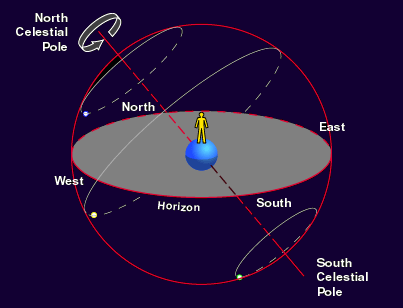
\includegraphics[width=\textwidth]{sphere-3.png}
\end{column}
\end{columns}
\bigskip
\bigskip
\Large
\color{A}A: I only \\
\color{B}B: II only \\
\color{C}C: III only \\
\color{D}D: I and II \\
\color{E}E: I, II, and III 
}


\frame{\frametitle{\textbf{Summary}}
\large
\BI
\item{We can treat the stars as all rotating together, on an invisible sphere far away}
\item{The axis of rotation is the same as the Earth's, and it rotates once per day}
\item{Only half of the sphere is visible, because the Earth is in the way}
\EI
\BC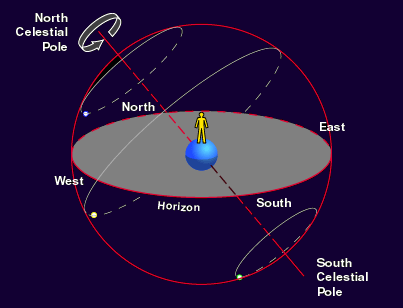
\includegraphics[width=0.5\textwidth]{sphere-3.png}\EC 
}
%
%\frame{
%\Large
%
%
%This picture was taken in Australia. Which way is the photographer looking?
%
%\bigskip
%\bigskip
%\begin{columns}
%\begin{column}{0.3\textwidth}
%\Huge
%\color{A}A: North \\
%\color{B}B: South \\
%\color{C}C: East \\
%\color{D}D: West \\
%\end{column}
%\begin{column}{0.7\textwidth}
%\BC
%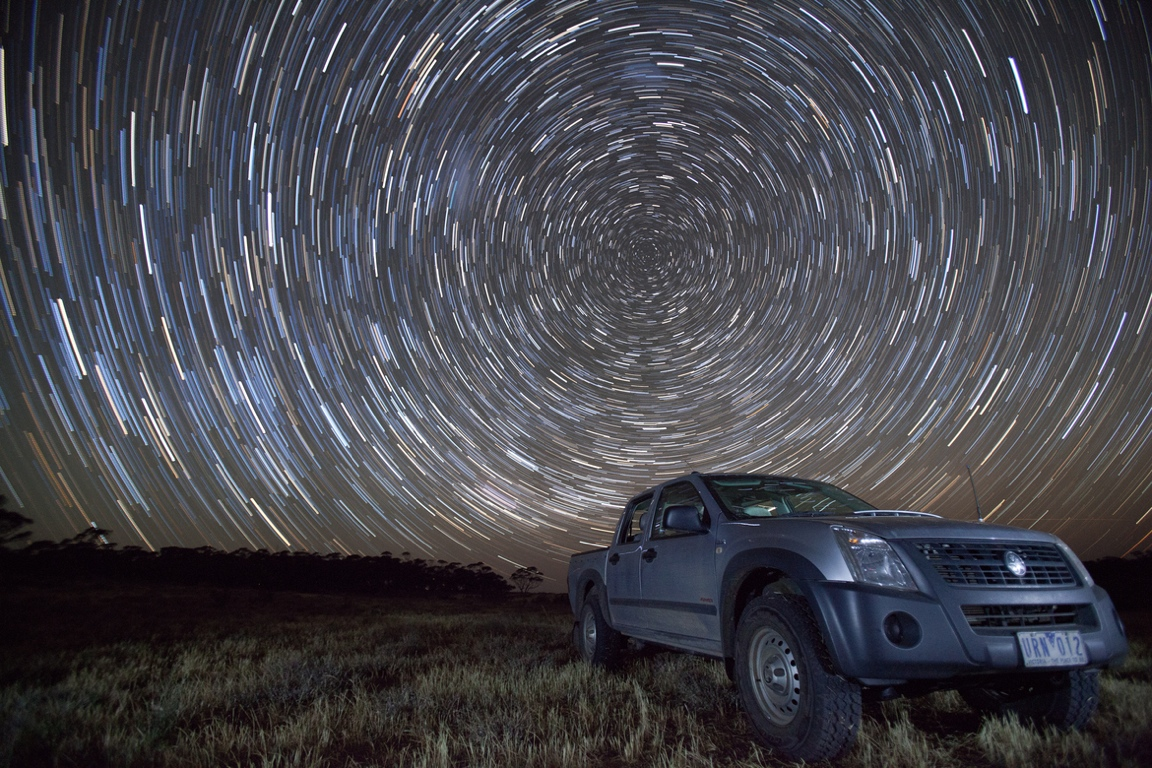
\includegraphics[width=\textwidth]{outback.jpg} \EC
%\end{column}
%\end{columns}
%}



\frame{
	\Large
	
	In Syracuse, you see this star at (A). Where will it be six hours later?
	
	\BC
	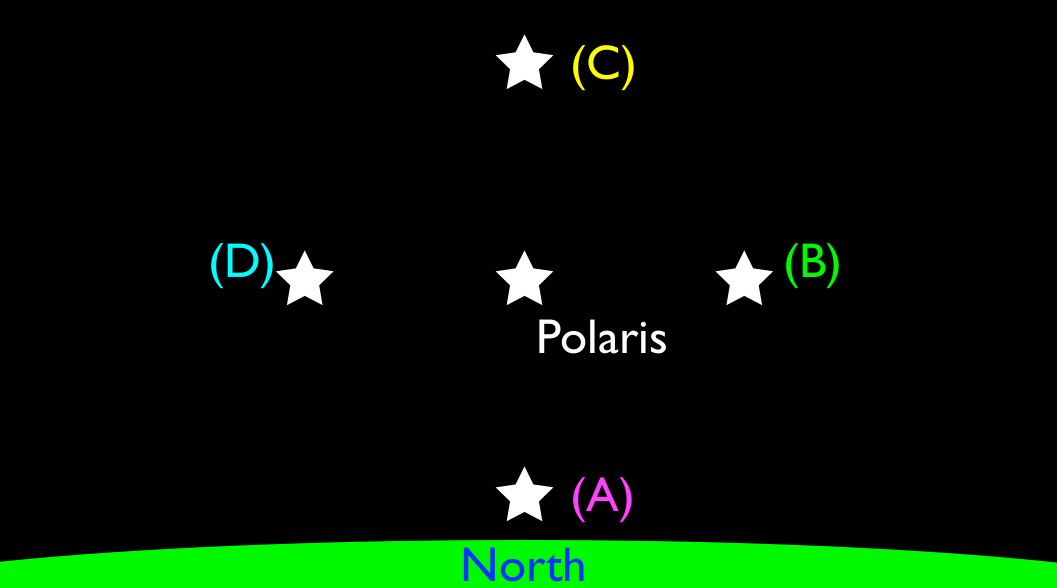
\includegraphics[width=0.8\textwidth]{star-question.png}
	\EC
}

\frame{
	\BC
	\Large
	How long is this star visible in the sky each day?
	\bigskip
	\bigskip
	
	\EC
	\begin{columns}
		\column{0.4\textwidth}
		\Large
		\color{A}A: All the time \\
		\color{B}B: More than 12 hours \\
		\color{C}C: Less than 12 hours \\
		\color{D}D: It's never visible  
		\column{0.6\textwidth}
		\BC
		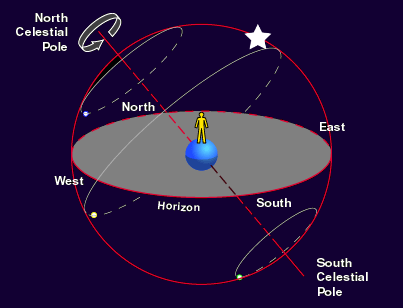
\includegraphics[width=0.95\textwidth]{how-long-2.png}
		\EC
	\end{columns}
	
}



\frame{\frametitle{\textbf{Tutorial from before}}
\Large
\BC
Take 10-15 minutes to complete the exercise from before. Then we will do something with your beach balls!
\EC
\BS\BS

\color{Red}Two things to note:

\BI
\item The reference to the ``camera'' on the bottom of the second page means ``the part of the simulation facing you''.

\BS\BS

\item There is an error on page 5 (section 2.3). \#3 should ask about the {\it green} star, not the purple one.
\EI

}


\frame{
	\BC
	\Large
	How long is this star visible in the sky each day?
	\bigskip
	\bigskip
	
	\EC
	\begin{columns}
		\column{0.4\textwidth}
		\Large
		\color{A}A: All the time \\
		\color{B}B: More than 12 hours \\
		\color{C}C: Less than 12 hours \\
		\color{D}D: It's never visible  
		\column{0.6\textwidth}
		\BC
		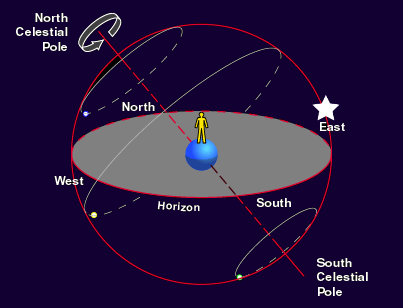
\includegraphics[width=0.95\textwidth]{how-long-3.png}
		\EC
	\end{columns}
	
}

\frame{
	\BC
	\Large
	How long is this star visible in the sky each day?
	\bigskip
	\bigskip
	
	\EC
	\begin{columns}
		\column{0.4\textwidth}
		\Large
		\color{A}A: All the time \\
		\color{B}B: More than 12 hours \\
		\color{C}C: Less than 12 hours \\
		\color{D}D: It's never visible  
		\column{0.6\textwidth}
		\BC
		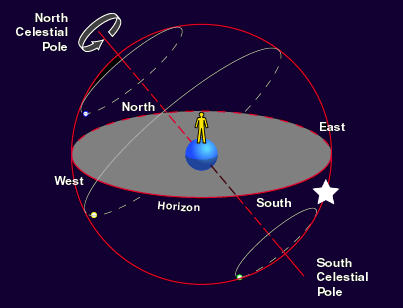
\includegraphics[width=0.95\textwidth]{how-long-4.png}
		\EC
	\end{columns}
	
}

\frame{

Let's look at our celestial sphere animation again.

\BS\pause

What's ``wrong'' with this model of the heavens?


}

\frame{\frametitle{\textbf{Problem 1: Depth and the sky}}
	\BC \Large The constellation of Orion:\EC
	
	\begin{columns}
		\begin{column}{0.5\textwidth}
			\BC 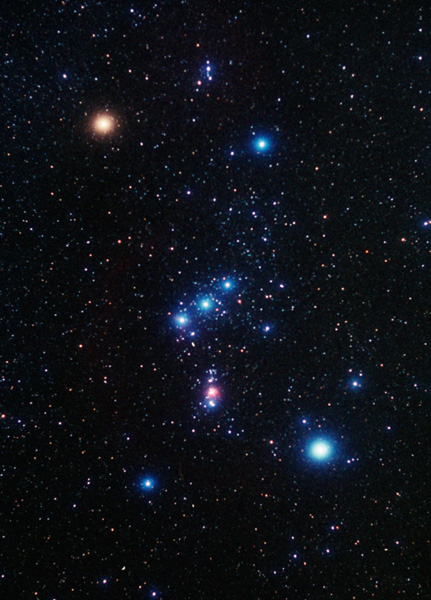
\includegraphics[width=0.8\textwidth]{orion-flat.jpg}\EC
		\end{column}
		\pause
		\begin{column}{0.5\textwidth}
			\BC 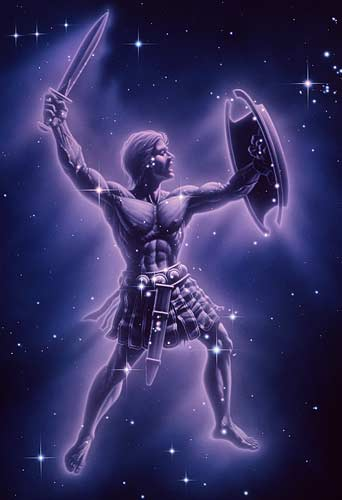
\includegraphics[width=0.8\textwidth]{orion-art.jpg}\EC
		\end{column}
	\end{columns}
}

\frame{\frametitle{\textbf{Problem 1: Depth and the sky}}
	\BC \Large The reality:\EC
	
	\bigskip
	\bigskip
	
	\BC 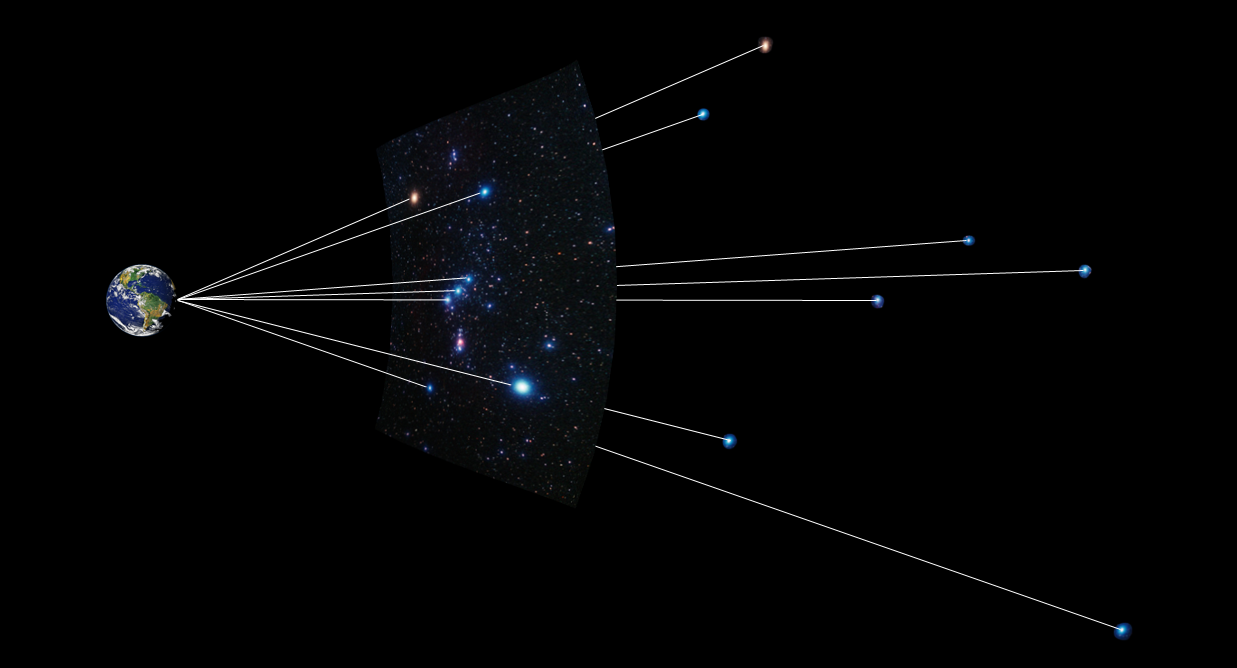
\includegraphics[width=0.9\textwidth]{orion-depth.png}\EC
}

\frame{\frametitle{\textbf{Problem 2: What's rotating?}}

\Large


The celestial sphere model proposes that (-------) rotates and (-------) stays still.

\pause\BS\BS

Really, though, we know that (-------) rotates and (-------) stays still.

\pause\BS\BS

Let's now figure out the motion of the stars with this knowledge.

}

\frame{
\huge

\BC
We'll start the Exercise together, then you should finish with the people around you.

\BS\BS

As always, raise your hand as you have questions!
\EC
\BS\BS

}

\frame{

\huge

\BC

There are two boxes by either exit of the auditorium.

\BS\BS

Please turn your homework in there. (It's the last page of the Exercise handout from last Thursday.)

\BS\BS\pause

Don't forget your prelabs for lab this week!

\BS\BS\pause

Be well, enjoy the beautiful fall weather, and I'll see you Thursday!
	
\EC
	
}

%
%
%\frame{
%
%\BC
%\Large
%Which star is visible longer?
%
%\bigskip
%\bigskip
%
%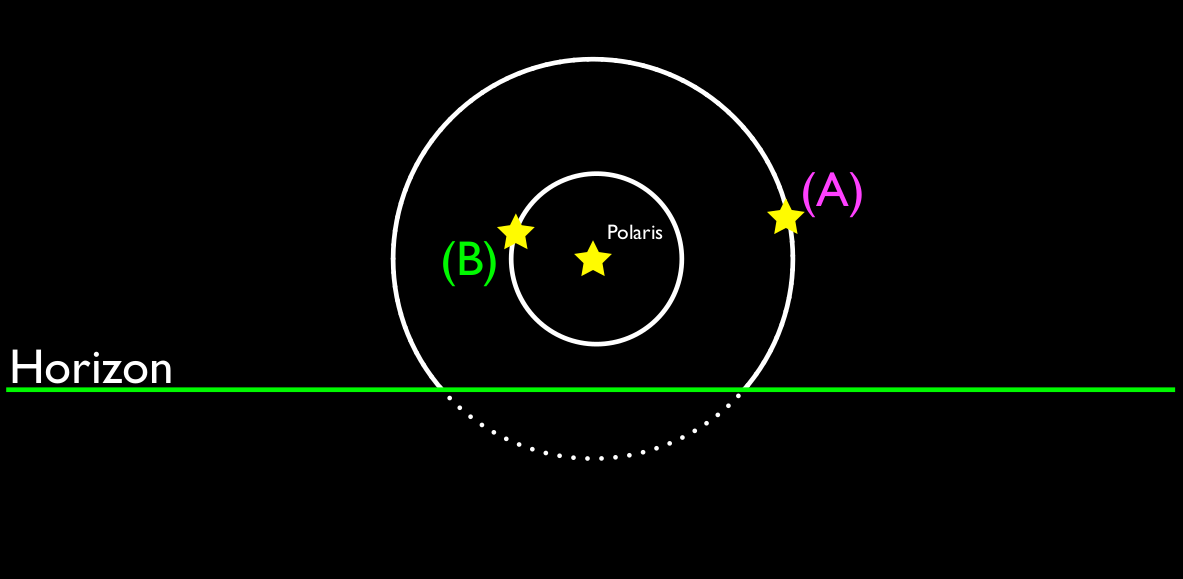
\includegraphics[width=0.8\textwidth]{visible-longer-1.png}
%\EC
%
%\pause\bigskip
%
%We call a star that is always above the horizon {\color{Red}circumpolar}.
%}	
%
%\frame{
%\BC
%\Large
%
%Where in the sky should I look to find circumpolar stars?
%
%\EC
%
%\BS\BS
%\color{A}A: High in the southern sky \\
%\color{B}B: Low in the eastern sky \\
%\color{C}C: High in the northern sky \\
%\color{D}D: Low-ish in the northern sky \\
%\color{E}E: Low in the northern sky \\
%}
%
%\frame{
%\Large
%\BC
%What about now? Which star is visible longer?
%
%\bigskip
%\bigskip
%
%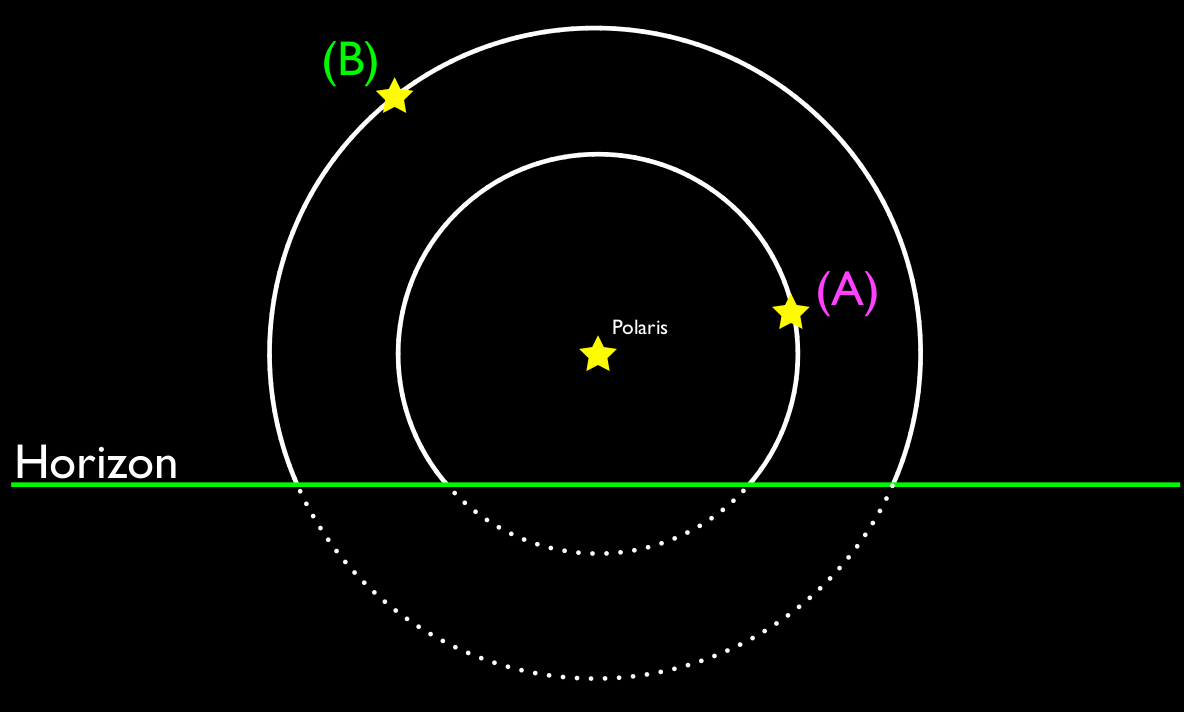
\includegraphics[width=0.8\textwidth]{visible-longer-2.png}
%\EC
%}	
%\frame{\frametitle{\textbf{What about the Sun?}}
%Over the course of one day, the Sun doesn't move very much.
%
%\bigskip
%\bigskip
%
%This means the celestial sphere model can show us how the Sun moves {\color{Red} each day}.
%
%\bigskip
%\bigskip
%
%It rises in the East and sets in the West, just like all the other stars.
%
%}
%
%\frame{
%\BC
%\Large
%How long is this star visible in the sky each day?
%\bigskip
%\bigskip
%
%\EC
%\begin{columns}
%\column{0.4\textwidth}
%\Large
%\color{A}A: All the time \\
%\color{B}B: More than 12 hours \\
%\color{C}C: Less than 12 hours \\
%\color{D}D: It's never visible  
%\column{0.6\textwidth}
%\BC
%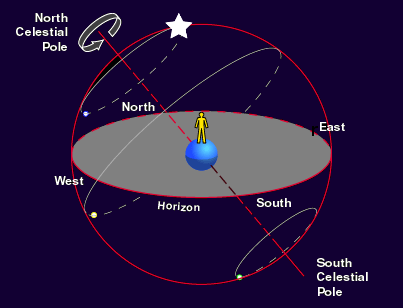
\includegraphics[width=0.95\textwidth]{how-long-1.png}
%\EC
%\end{columns}
%
%}
%
%
%
%\frame{\frametitle{\textbf{What does one star matter?}}
%\Large
%The visibility of one star in our sky isn't that big of a deal...
%
%\pause
%\bigskip
%\bigskip
%
%... unless that star is the Sun! We'll talk about this Thursday.
%}



\end{document}
